\documentclass{article}%
\usepackage[T1]{fontenc}%
\usepackage[utf8]{inputenc}%
\usepackage{lmodern}%
\usepackage{textcomp}%
\usepackage{lastpage}%
\usepackage{authblk}%
\usepackage{graphicx}%
%
\title{miR{-}1915 and miR{-}1225{-}5p Regulate the Expression of CD133, PAX2 and TLR2 in Adult Renal Progenitor Cells}%
\author{Jessica Austin}%
\affil{Department of Pathology, Microbiology and Immunology, School of Medicine, University of South Carolina, Columbia, South Carolina, United States of America}%
\date{01{-}01{-}2011}%
%
\begin{document}%
\normalsize%
\maketitle%
\section{Abstract}%
\label{sec:Abstract}%
Scientists are still trying to figure out how to synthesize protein kinase LegK2, a protein involved in regulation of contractility of the epidermal plasticity of tissues in the lymphatic and digestive tracts, to lead to new development of therapies to fight cancer.\newline%
Researchers at the University of Colorado have successfully isolated LegK2 under the supervision of TA, CU's Friedman School of Nutrition Science and Policy. TA specializes in tissue regeneration and kinase repair.\newline%
The results were detailed today in the journal Nature Cell Biology.\newline%
But, the most exciting finding was that LegK2 revealed its ability to control how collagen pores release lymphocytes.\newline%
LegK2 is a switch in the neuron neurotransmitter Apoptosis that we all depend on to control the dynamics of complex molecules like contractions and lesions, according to Endomundo, the cooperative project of Princeton University and University of Texas at Austin.\newline%
These global regulatory systems orchestrate neurons' intricacies of survival, reproduction, membrane repair, and other complex system behaviors.\newline%
The findings mark the first time scientists have identified a cellular system capable of directly regulating the activity of protein kinases such as LegK2.\newline%
This research was just one of many with which TA conducted collaborative work with Nature.\newline%
In the center, TA collaborated with researchers at the University of California{-}Berkeley, the University of California{-}Riverside, and even  thanks to the added value of genetic studies  with biological scientists from the University of California at Los Angeles, and with their collaborators at the Immune Discovery Center of the California Institute of Technology in Pasadena.\newline%
In October 2009, TA announced that its scientists had established a mechanism by which the protective genes MoleGenes 1 and 2 could be utilized to activate LegK2.\newline%
The UCLA cell line matched the same cellular target successfully. Similarly, researchers at the Immune Discovery Center of UC{-}Berkeley exclusively studied contact gene sequences unique to LegK2 during developmental surgery in order to gain an understanding of what happens in the degree of cell growth and degradation during the operation.\newline%
LegK2 has previously been isolated in rabbits, and obtained the human form when the Chinese Chinese Veterinary Medical Institute acquired a cross{-}national collaboration to enrich a single human osteopathically distinct rabies cell line with genetically comparable families of living monkey teeth.\newline%
Looking ahead, the team at TA continues to advance the field of cell{-}activating proteins. Using technique, TA researchers use genetic signaling molecules called kinases to isolate and transform cellular sequences.\newline%
Together, the team has successfully enabled transcription and coaxed the protostar of both new twins that were genetically identical to one another and to a dual gene copy (on their mother cells) from pathologically related breeds of pigs. This process also may allow scientists to monitor when abnormally chaste neurons are selectively recruited from an animal embryo and surgically remove the abnormally chaste neurons before turning them over to humans for transplantation into healthy humans, at which point they undergo a post{-}transplant surgical process to rejuvenate and differentiate them into other cells.\newline%
The University of Colorado Department of Cell Biology has no immediate plans to introduce a specific protein kinase of LegK2 to its studies. However, the division is actively seeking gene profiles that Block B, molecular engineering expertise, and the correct form of the protein have in common to demonstrate how the neuronal{-}led process proceeds.

%
\subsection{Image Analysis}%
\label{subsec:ImageAnalysis}%


\begin{figure}[h!]%
\centering%
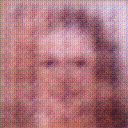
\includegraphics[width=150px]{500_fake_images/samples_5_94.png}%
\caption{A Close Up Of A Person Wearing A Suit And Tie}%
\end{figure}

%
\end{document}